\documentclass[acmsmall]{acmart}

\def\BibTeX{{\rm B\kern-.05em{\sc i\kern-.025em b}\kern-.08emT\kern-.1667em\lower.7ex\hbox{E}\kern-.125emX}}
    
\copyrightyear{2019}
\acmYear{2019}
\setcopyright{acmlicensed}
\acmConference[Woodstock '18]{Woodstock '18: ACM Symposium on Neural Gaze Detection}{June 03--05, 2018}{Woodstock, NY}
\acmBooktitle{Woodstock '18: ACM Symposium on Neural Gaze Detection, June 03--05, 2018, Woodstock, NY}
\acmPrice{15.00}
\acmDOI{10.1145/1122445.1122456}
\acmISBN{978-1-4503-9999-9/18/06}

\begin{document}

%
% The "title" command has an optional parameter, allowing the author to define a "short title" to be used in page headers.
\title{Functional Perl: Functional Reactive Patterning with TidalCycles}

\author{Alex McLean}
% \authornote{Both authors contributed equally to this research.}
\email{alex@slab.org}
\orcid{0000-0002-7428-7935}
\affiliation{%
  \institution{Deutsches Museum}
  \streetaddress{Museuminsel 1}
  \city{Munich}
  \state{Bavaria}
  \postcode{80538}
}

%
% By default, the full list of authors will be used in the page headers. Often, this list is too long, and will overlap
% other information printed in the page headers. This command allows the author to define a more concise list
% of authors' names for this purpose.
% \renewcommand{\shortauthors}{Trovato and Tobin, et al.}

%
% The abstract is a short summary of the work to be presented in the article.
\begin{abstract}
Abstract goes here
\end{abstract}

%
% The code below is generated by the tool at http://dl.acm.org/ccs.cfm.
% Please copy and paste the code instead of the example below.
%

\begin{CCSXML}
<ccs2012>
<concept>
<concept_id>10010405.10010469.10010471</concept_id>
<concept_desc>Applied computing~Performing arts</concept_desc>
<concept_significance>500</concept_significance>
</concept>
<concept>
<concept_id>10010405.10010469.10010475</concept_id>
<concept_desc>Applied computing~Sound and music computing</concept_desc>
<concept_significance>500</concept_significance>
</concept>
<concept>
<concept_id>10011007.10011006.10011008.10011009.10011012</concept_id>
<concept_desc>Software and its engineering~Functional languages</concept_desc>
<concept_significance>500</concept_significance>
</concept>
<concept>
<concept_id>10011007.10011006.10011050.10011017</concept_id>
<concept_desc>Software and its engineering~Domain specific languages</concept_desc>
<concept_significance>500</concept_significance>
</concept>
</ccs2012>
\end{CCSXML}

\ccsdesc[500]{Applied computing~Performing arts}
\ccsdesc[500]{Applied computing~Sound and music computing}
\ccsdesc[500]{Software and its engineering~Functional languages}
\ccsdesc[500]{Software and its engineering~Domain specific languages}

\keywords{functional reactive programming, live coding, haskell, pattern}

%
% A "teaser" image appears between the author and affiliation information and the body 
% of the document, and typically spans the page. 
%%\begin{teaserfigure}
%%  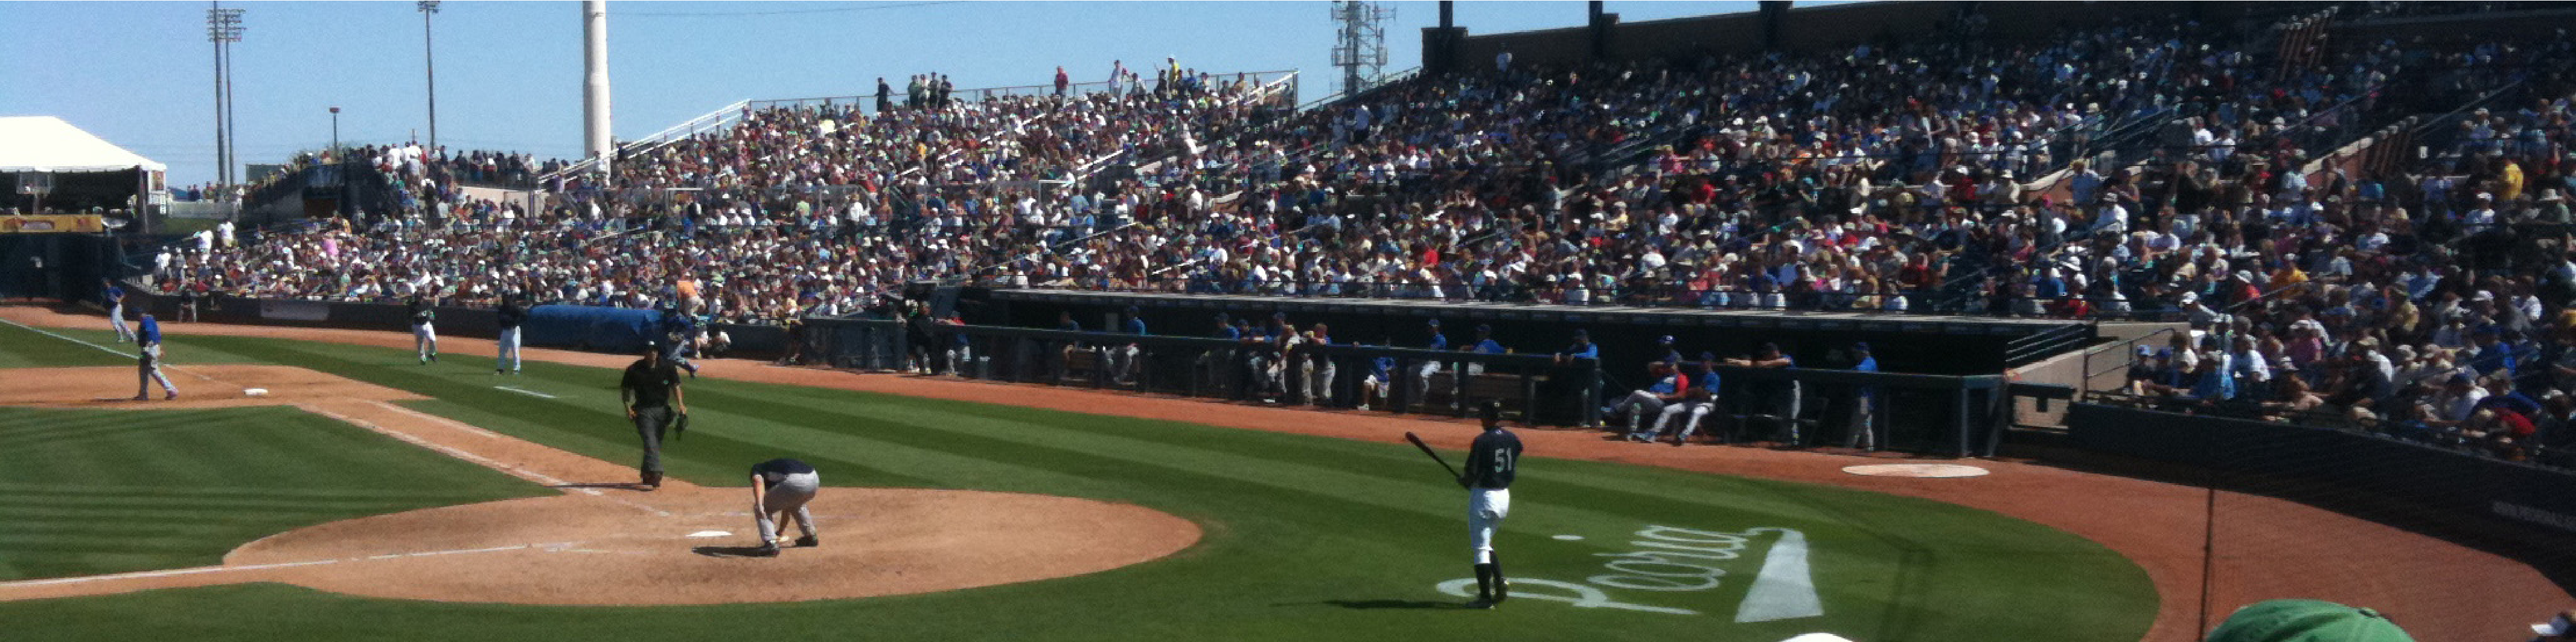
\includegraphics[width=\textwidth]{sampleteaser}
%%  \caption{Seattle Mariners at Spring Training, 2010.}
%%  \Description{Enjoying the baseball game from the third-base seats. Ichiro Suzuki preparing to bat.}
%%  \label{fig:teaser}
%%\end{teaserfigure}

\maketitle

\section{Introduction}

TidalCycles (or commonly \emph{Tidal} for short) is a domain specific
language (DSL) for creating patterns, implemented in the Haskell
programming language. \emph{Pattern} here is used in the same sense as
in textiles; ways of creating results through a series of patterning
operations such as repetition, reflection, rotation, combination,
interference and randomisation.

Tidal has been developed over a number of years, for the first few
used only by myself, but is now a thriving free/open source project,
with people using it to make music around the world. It does not
itself make sound, and can be easily decoupled from the default
``SuperDirt'' synthesiser, and has been used to pattern live video,
solenoids hitting drums, lights over the DMX protocol, woven textiles,
and even choreographic instructions.

While Tidal has been developed alongside creative practice, it upholds
strong computer scientific principles. Crucially, a pattern is defined
as a pure function, and therefore may be combined flexibly and safely.
Tidal is often live coded, where the performer must make changes
quickly and without runtime errors. As Tidal has developed, its core
representation has grown more succinct, and a recent rewrite resulted
in more rigorous understanding of what, in terms of Tidal, a pattern
\emph{is}. The following paper communicates this result, and explains
the key parts of Tidal's combinator library in order to get across its
usefulness.

\section{Tidal patterns}



\begin{acks}
ERC
\end{acks}

\bibliographystyle{ACM-Reference-Format}
\bibliography{alex.bib}

\end{document}
